\documentclass[a4paper,12p]{article}
\usepackage[utf8]{inputenc}
\usepackage[ngerman]{babel}
\usepackage[a4paper, left=2.5cm, right=2.5cm]{geometry}
\usepackage{amsmath}
\usepackage{graphicx}

\title{\huge Modellbildung\\\large \huge Beispielsammlung}
\author{\huge 4.Semester ET-Studium}
\date{\huge November 2018}
\begin{document}	
\maketitle
\newpage
\tableofcontents
\newpage
\section{Einleitung}
Die Modellbildung beschäftigt sich mit der mathematischen Beschreibung von Systemen, um diese dann beispielsweise mit Hilfe eines Reglers zu automatisieren.
\newline
Der Inhalt dieser Ausarbeitung beinhaltet nur die Aufgaben, aus dem Skript der Vorlesung der Modellbildung, welche eine Pflichtlehrveranstaltung im 4.Semester im Bachelor-Studium der Elektrotechnik ist. Der Lösungsweg der hier erwähnten Beispiele wird im Skript nicht explizit ausgearbeitet. Variablen der Form \textbf{x} sind Vektoren und der Form \textbf{A} sind Matrizen. \\
Die Ausarbeitung enthält nur die Beispiele die ohne nötiger Hilfe von Maple gelöst werden können und wo man keine mathematischen Beweise durchführen muss.
\section{Mechanische Systeme}
\subsection{Punkt-Kinematik}
\textbf{\textit{\underline{Aufgabe 2.1}}}
\newline\newline
 Zeigen Sie, dass sich die Geschwindigkeitskomponenten eines materiellen Punktes \textit{P} im Raum bezüglich der normierten Basisvektoren $ e_{r} , e_{\theta} $ und $ e_{\varphi} $ in Kugelkoordinaten
 \begin{equation*}
 	x = r\sin(\theta)\cos(\varphi),\qquad y = r\sin(\theta)\sin(\varphi),\qquad z = r\cos(\theta)
 \end{equation*}
 zu
 \begin{equation*}
 	v_{r} = \dot{r},\qquad v_{\theta} = r\dot{\theta},\qquad v_{\varphi} = r\sin(\theta)\dot{\varphi}
 \end{equation*}
 errechnen.
 \newline\newline
 \textbf{Lösungsweg:}
 \newline\newline
 Die Geschwindigkeit mit der Form
 \begin{equation*}
 	\textbf{v}_{t} = v_{x}\textbf{e}_{x} + v_{y}\textbf{e}_{y} + v_{z}\textbf{e}_{z} = \dot{x}\textbf{e}_{x} + \dot{y}\textbf{e}_{y} + \dot{z}\textbf{e}_{z}
 \end{equation*}
 erhält man, durch die Anwendung der Kettenregel der Differentiation hier mit der Form
 \begin{equation*}
 	\textbf{v}(t) = \left(\frac{\partial}{\partial r}\textbf{r}\right) \dot{r} \ + \ \left(\frac{\partial}{\partial \varphi}\textbf{r}\right)  \dot{\varphi} \ + \ \left(\frac{\partial}{\partial \theta}\textbf{r}\right)\dot{\theta}
 \end{equation*}
 Die Basisvektoren bilden sich folgendermaßen aus
 \begin{align*}
 	\tilde{\textbf{e}}_{r} & = \sin(\theta)\cos(\varphi)\textbf{e}_{x} \ + \ \sin(\theta)\sin(\varphi)\textbf{e}_{y} \ + \ \cos(\theta)\textbf{e}_{z} \\ 
 	\tilde{\textbf{e}}_{\theta} & = r\cos(\theta)\cos(\varphi)\textbf{e}_{x} \ + \ r\cos(\theta)\sin(\varphi)\textbf{e}_{y} \ - \ r\sin(\theta)\textbf{e}_{z} \\
 	\tilde{\textbf{e}}_{\varphi} & = -r\sin(\theta)\sin(\varphi)\textbf{e}_{x} \ + \ r\sin(\theta)\cos(\varphi)\textbf{e}_{y} 	
 \end{align*}
 Diese Vektoren können nur dann eine zulässige Basis eines Koordinatensystems sein, wenn die Matrix
\begin{equation*}
	\textbf{J} =
	 \begin{bmatrix}
	 	\sin(\theta)\cos(\varphi) & \sin(\theta)\sin(\varphi) & \cos(\theta) \\
	 	r\cos(\theta)\cos(\varphi) & r\cos(\theta)\sin(\varphi) & -r\sin(\theta) \\
	 	-r\sin(\theta)\sin(\varphi) & r\sin(\theta)\cos(\varphi) & 0
	 \end{bmatrix}
\end{equation*}
\\
regulär ist. D.h. die Determinante dieser Matrix muss $\neq 0$  sein.
Die Matrix \textbf{J} wird folgendermaßen gefüllt: \\
\begin{equation*}
	\textbf{J} = 
		\begin{bmatrix}
			x_r & y_r & z_r \\
			x_\theta & y_\theta & z_\theta \\
			x_\varphi & y_\varphi & z_\varphi \\
		\end{bmatrix}
\end{equation*}
Hier det(\textbf{J}) = $r\sin\theta \neq 0$ wenn $r \neq 0$ und es gilt $\theta: [0,\frac{\pi}{2}]$ $\Rightarrow$ det(\textbf{J}) $\in$ regulär.\\
\underline{Beweis:} \\
Da es sich hier um eine $ 3 \times 3 $-Matrix handelt kann die Determinante dieser Matrix mithilfe des Satzes von Sarus gelöst werden.
\begin{align*}
	det(\textbf{J}) & = r^2\sin^3(\theta)\sin^2(\varphi) + r^2\cos^2(\theta)\cos^2(\varphi)\sin(\theta) + r^2\cos^2(\theta)\sin^2(\varphi)\sin(\theta) + r^2\sin^3(\theta)\cos^2(\varphi) =\\
	& = r^2(\sin^3(\theta)\sin^2(\varphi) + \cos^2(\theta)\cos^2(\varphi)\sin(\theta) + \cos^2(\theta)\sin^2(\varphi)\sin(\theta) + \sin^3(\theta)\cos^2(\varphi)) =\\
	& = r^2(\cos^2(\theta)\cos^2(\varphi)\sin(\theta) + \cos^2(\theta)\sin^2(\varphi)\sin(\theta) + \sin^3(\theta)(\sin^2(\varphi) + \cos^2(\varphi)) =\\
	& = r^2(\cos^2(\theta)\cos^2(\varphi)\sin(\theta) + \cos^2(\theta)\sin^2(\varphi)\sin(\theta) + \sin^3(\theta)) =\\
	& = r^2(\sin^3(\theta) + \cos^2(\theta)\sin(\theta)(\cos^2(\varphi) + \sin^2(\varphi))) =\\
	& = r^2(\sin^3(\theta) + \cos^2(\theta)\sin(\theta)) =\\
	& = r^2(\sin(\theta)\sin^2(\theta) + \cos^2(\theta)\sin(\theta)) = \\
	& = r^2(\sin(\theta)(\sin^2(\theta) + \cos^2(\theta))) = \\
	& = r^2\sin(\theta) \\ \\
	det(\textbf{J}) & = r^2\sin(\theta)
\end{align*}
Anschließend muss man die gerade ermittelten Basisvektoren normieren.\newline
Die Längen der Vektoren $\tilde{\textbf{e}}_{r},\tilde{\textbf{e}}_{\varphi}$ und $\tilde{\textbf{e}}_{\theta}$ betragen $1,r\sin\theta$ und $r$.
\newline
Normierte Basisvektoren:
\begin{align*}
	\textbf{e}_{r} & = \sin(\theta)\cos(\varphi)\textbf{e}_{x} \ + \ \sin\theta)\sin(\varphi)\textbf{e}_{y} \ + \ \cos(\theta)\textbf{e}_{z} \\
	\textbf{e}_{\theta} & = \cos(\theta)\cos(\varphi)\textbf{e}_{x} \ + \ \cos(\theta)\sin(\varphi)\textbf{e}_{y} \ - \sin(\theta)\textbf{e}_{z} \\
	\textbf{e}_{\varphi} & = -\sin(\varphi)\textbf{e}_{x} \ + \ \cos(\varphi)\textbf{e}_{y}
\end{align*}
Mit diesen Basisvektoren lässt sich die Geschwindigkeit in der Form
\begin{equation*}
	\textbf{v}(t) = v_{r}\textbf{e}_{r} + v_{\theta}\textbf{e}_{\theta} + v_{\varphi}\textbf{e}_{\varphi} = \dot{r}\textbf{e}_{r} + r\dot{\theta}\textbf{e}_{\theta} +  r\sin(\theta)\dot{\varphi}\textbf{e}_{\varphi}
\end{equation*}
darstellen.
\begin{equation*}
	v_r = \dot{r} \ , \ v_\theta = r\dot{\theta} \ , \ v_\varphi = r\sin(\theta)\dot{\varphi}
\end{equation*}
\newpage
\subsection{Newtonsche Gesetze}
\subsubsection{Kräftesystem}
\textbf{\textit{\underline{Aufgabe 2.3}}} \\ \\
Ein vertikaler Mast M wird gemäß der Abbildung durch Seile abgespannt.
\begin{figure}[h]
\begin{center}
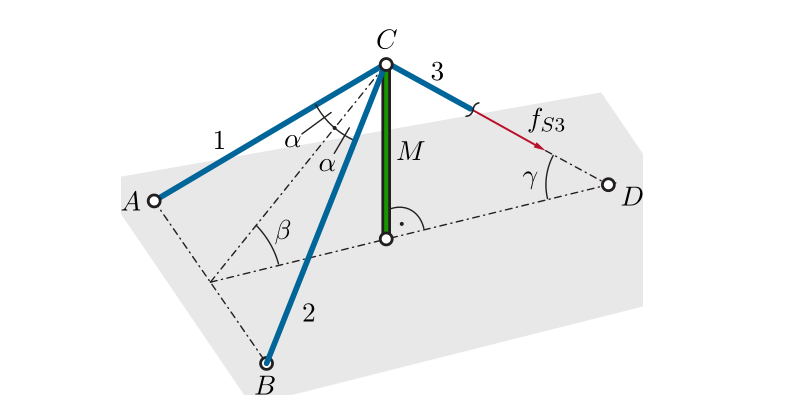
\includegraphics[width=12.5cm]{pic/Angabe}
\caption{Angabe Aufgabe 2.3}
\label{Angabe}
\end{center}
\end{figure} \\
Wie groß sind die Kräfte $ f_{s1} $ und $ f_{s2} $ in den Seilen 1 und 2 und die Kraft $ f_M $ im Mast, wenn am Seil 3 die Zugkraft $ f_{s3} $ aufgebracht wird? \\ \\
\textbf{Lösungsweg:} \\ \\
Zunächst müssen die Gleichungen für die Gleichgewichtsbedingung aufgestellt werden. Da sich es in Abbildung \ref{Angabe} um ein 3-dimensionales Beispiel handelt muss man die Gleichgewichtsbedingung für alle drei Raumrichtungen aufstellen.
\begin{align*}
	(1) \ \ \ e_x & : f_{s1}\cos(\alpha) - f_{s2}\cos(\alpha) = 0 \\
	(2) \ \ \ e_y & : f_{s3}\cos(\gamma) - f_{s1}\cos(\alpha)\cos(\beta) - f_{s2}\cos(\alpha)\cos(\beta) = 0 \\  
	(3) \ \ \ e_z & : -f_M - f_{s3}\sin(\gamma) - f_{s2}\cos(\alpha)\sin(\beta) - f_{s1}\cos(\alpha)\sin(\beta) = 0
\end{align*}
Nun hat man ein einfaches Gleichungssystem mit 3 Gleichungen, welches nach diesen auch gelöst werden soll. Als erstes formt man die Gleichung (1) auf $f_{s1}$ um. \\ 
Hieraus folgt:
\begin{equation*}
	f_{s1} = f_{s2}
\end{equation*}
Im nächsten Schritt setzt man die umgeformte Gleichung (1) in Gleichung (2) ein und formt diese auf $ f_{s1} $ um. \\
Hieraus folgt:
\begin{align*}
	f_{s3}&\cos(\gamma) - f_{s1}\cos(\alpha)\cos(\beta) - f_{s1}\cos(\alpha)\cos(\beta) = 0 \\
	f_{s3}&\cos(\gamma) - 2f_{s1}\cos(\alpha)\cos(\beta) = 0 \\
	f_{s1}&=f_{s2} = \frac{f_{s3}\cos(\gamma)}{2\cos(\alpha)\cos(\beta)}
\end{align*}

loaoaoaool
\end{document}
